\documentclass[tikz,border=8pt]{standalone}
% Shared look for every TikZ diagram. Load with % Shared look for every TikZ diagram. Load with % Shared look for every TikZ diagram. Load with \input{../../tools/tikz-style.tex}
\usepackage[T1]{fontenc}
\usepackage{lmodern}
\renewcommand{\sfdefault}{lmr}  % diagrams use the same serif as the text
\usetikzlibrary{arrows.meta, positioning, shapes.geometric, calc, fit, backgrounds}
\definecolor{cblue}{HTML}{4C78A8}
\definecolor{corange}{HTML}{F58518}
\definecolor{cgreen}{HTML}{54A24B}
\definecolor{cred}{HTML}{E45756}
\definecolor{cpurple}{HTML}{B279A2}
\definecolor{cgrey}{HTML}{6B6B6B}
\tikzset{
  every picture/.style={font=\sffamily, line width=1.2pt},
  box/.style={draw=#1, fill=#1!12, rounded corners=4pt, align=center, inner sep=7pt, minimum height=1.1cm},
  box/.default=cgrey,
  arrow/.style={-{Stealth[length=3mm]}, draw=cgrey, line width=1.4pt},
  title/.style={font=\sffamily\bfseries\Large},
  note/.style={font=\sffamily\small, text=cgrey, align=center},
}
\AtBeginDocument{\hyphenpenalty=10000 \exhyphenpenalty=10000}

\usepackage[T1]{fontenc}
\usepackage{lmodern}
\renewcommand{\sfdefault}{lmr}  % diagrams use the same serif as the text
\usetikzlibrary{arrows.meta, positioning, shapes.geometric, calc, fit, backgrounds}
\definecolor{cblue}{HTML}{4C78A8}
\definecolor{corange}{HTML}{F58518}
\definecolor{cgreen}{HTML}{54A24B}
\definecolor{cred}{HTML}{E45756}
\definecolor{cpurple}{HTML}{B279A2}
\definecolor{cgrey}{HTML}{6B6B6B}
\tikzset{
  every picture/.style={font=\sffamily, line width=1.2pt},
  box/.style={draw=#1, fill=#1!12, rounded corners=4pt, align=center, inner sep=7pt, minimum height=1.1cm},
  box/.default=cgrey,
  arrow/.style={-{Stealth[length=3mm]}, draw=cgrey, line width=1.4pt},
  title/.style={font=\sffamily\bfseries\Large},
  note/.style={font=\sffamily\small, text=cgrey, align=center},
}
\AtBeginDocument{\hyphenpenalty=10000 \exhyphenpenalty=10000}

\usepackage[T1]{fontenc}
\usepackage{lmodern}
\renewcommand{\sfdefault}{lmr}  % diagrams use the same serif as the text
\usetikzlibrary{arrows.meta, positioning, shapes.geometric, calc, fit, backgrounds}
\definecolor{cblue}{HTML}{4C78A8}
\definecolor{corange}{HTML}{F58518}
\definecolor{cgreen}{HTML}{54A24B}
\definecolor{cred}{HTML}{E45756}
\definecolor{cpurple}{HTML}{B279A2}
\definecolor{cgrey}{HTML}{6B6B6B}
\tikzset{
  every picture/.style={font=\sffamily, line width=1.2pt},
  box/.style={draw=#1, fill=#1!12, rounded corners=4pt, align=center, inner sep=7pt, minimum height=1.1cm},
  box/.default=cgrey,
  arrow/.style={-{Stealth[length=3mm]}, draw=cgrey, line width=1.4pt},
  title/.style={font=\sffamily\bfseries\Large},
  note/.style={font=\sffamily\small, text=cgrey, align=center},
}
\AtBeginDocument{\hyphenpenalty=10000 \exhyphenpenalty=10000}

\begin{document}
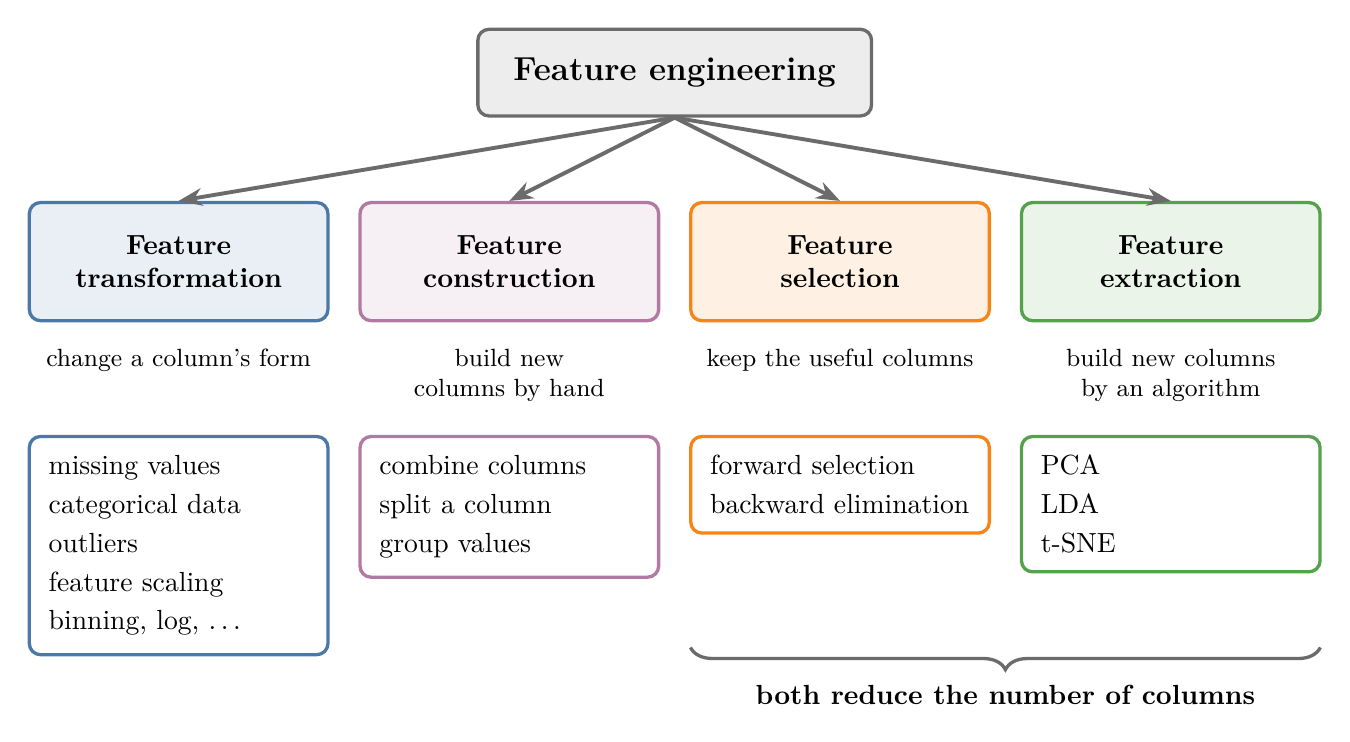
\begin{tikzpicture}
  \node[box=cgrey, font=\sffamily\bfseries\large, minimum width=5cm] (fe) at (6.3,0) {Feature engineering};
  \foreach \x/\n/\c/\t in {0/t/cblue/Feature\\transformation, 4.2/c/cpurple/Feature\\construction, 8.4/s/corange/Feature\\selection, 12.6/e/cgreen/Feature\\extraction} {
    \node[box=\c, font=\sffamily\bfseries, text width=3.3cm, minimum height=1.5cm] (\n) at (\x,-2.4) {\t};
    \draw[arrow] (fe.south) -- (\n.north);
  }
  \node[note, below=0.2cm of t, text=black, text width=3.6cm] {change a column's form};
  \node[note, below=0.2cm of c, text=black, text width=3.6cm] {build new columns by hand};
  \node[note, below=0.2cm of s, text=black, text width=3.6cm] {keep the useful columns};
  \node[note, below=0.2cm of e, text=black, text width=3.6cm] {build new columns\\by an algorithm};
  % techniques
  \node[box=cblue, fill=white, align=left, text width=3.3cm, anchor=north] at (0,-4.6)
    {missing values\\[2pt] categorical data\\[2pt] outliers\\[2pt] feature scaling\\[2pt] binning, log, \dots};
  \node[box=cpurple, fill=white, align=left, text width=3.3cm, anchor=north] at (4.2,-4.6)
    {combine columns\\[2pt] split a column\\[2pt] group values};
  \node[box=corange, fill=white, align=left, text width=3.3cm, anchor=north] at (8.4,-4.6)
    {forward selection\\[2pt] backward elimination};
  \node[box=cgreen, fill=white, align=left, text width=3.3cm, anchor=north] at (12.6,-4.6)
    {PCA\\[2pt] LDA\\[2pt] t-SNE};
  \draw[decorate, decoration={brace, amplitude=8pt, mirror}, draw=cgrey]
    (6.5,-7.3) -- (14.5,-7.3) node[midway, below=10pt, font=\sffamily\bfseries] {both reduce the number of columns};
\end{tikzpicture}
\end{document}
